%! TeX program = lualatex
\documentclass[12pt,a4paper]{article}

\usepackage[nil]{babel}
\usepackage{unicode-math}
\usepackage[svgnames]{xcolor}
\usepackage{lmodern}
\usepackage{graphicx}
\usepackage{wrapfig}
\usepackage{float}
\usepackage{parskip}
\usepackage{xurl}
\usepackage[font=small,labelfont=bf,justification=centering]{caption}

\babelprovide[import=el, main, onchar=ids fonts]{greek} % can also do import=el-polyton
\babelprovide[import, onchar=ids fonts]{english}

\babelfont{rm}
          [Language=Default]{Liberation Sans}
\babelfont[english]{rm}
          [Language=Default]{Liberation Sans}
\babelfont{sf}
          [Language=Default]{Liberation Sans}
\babelfont{tt}
          [Language=Default]{Liberation Sans}

\renewcommand{\thesubsection}{\thesection.\alph{subsection}}
\setlength{\emergencystretch}{3em}

%Enter Title Here
\title{Εργασία Υπολογιστική Νοημοσύνη\\Μέρος Α}
\author{Γρηγόρης Καπαδούκας (ΑΜ: 1072484)}

\begin{document}
\maketitle

\setcounter{section}{-1}
\section{Περιβάλλον Εργασίας - Σύνδεσμος GitHub με Κώδικα}
Για την διεκπεραίωση αυτής της εργασίας έχω επιλέξει να χρησιμοποιήσω γλώσσα προγραμματισμού Python μαζί τις βιβλιοθήκες TensorFlow (κυρίως το API της, το Keras) για τον σχεδιασμό και την εκπαίδευση των νευρωνικών δικτύων. Επίσης χρησιμοποιώ Pandas και Scikit-Learn με σκοπό τον χειρισμό του CSV αρχείου και της προεπεξεργασίας.

Ο κώδικας που γράφτηκε για την εργασία βρίσκεται στο repository στον παρακάτω σύνδεσμο:

\textcolor{blue}{\url{https://github.com/GregKapadoukas/University-Computational-Intelligence-Project-A}}
\section{Προεπεξεργασία και Προετοιμασία Δεδομένων}

\subsection{Κωδικοποίηση και προεπεξεργασία δεδομένων}

\subsubsection{Διάβασμα του CSV αρχείου και μετατροπή κατηγορικών δεδομένων σε αριθμητικά}
Αρχικά, με σκοπό το διάβασμα του dataset στη μορφή του CSV αρχείου χρησιμοποιώ εντολές της βιβλιοθήκης Pandas για φορτώσω τα δεδομένα στη μορφή ενός DataFrame. Έπειτα χωρίζω το αρχικό DataFrame σε δύο, από τα οποία το πρώτο περιέχει τα δεδομένα των αισθητήρων και τα στοιχεία του ατόμου πάνω στο οποίο έγιναν οι μετρήσεις και το δεύτερο περιέχει την κλάση δραστηριότητας στην οποία ανήκει το άτομο.

Έπειτα μετατρέπω τα κατηγορικά δεδομένα των κλάσεων του δεύτερου DataFrame σε αριθμητικά δεδομένα, τα οποία όμως είναι one-hot encoded διανύσματα μεγέθους $\mathbb{R}\textsuperscript{1\times5}$. Άρα οι τιμές μετατρέπονται σε διανύσματα με την εξής αντιστοίχηση:

\begin{itemize}
    \item 'sitting': [1 0 0 0 0]
    \item 'sitting-down': [0 1 0 0 0]
    \item 'standing': [0 0 1 0 0]
    \item 'standing-up': [0 0 0 1 0]
    \item 'walking': [0 0 0 0 1]
\end{itemize}

Επέλεξα την παραπάνω one-hot encoded προσέγγιση αντί για την αριθμητική 1-5 όπως προτείνεται στην εκφώνηση, επειδή σκοπεύω να έχω 5 εξόδους στο νευρωνικό δίκτυο, όπως θα εξηγήσω στο κεφάλαιο \ref{Επιλογή Αρχιτεκτονικής}.

Έπειτα μετατρέπω και τα κατηγορικά δεδομένα του δεύτερου DataFrame, δηλαδή τα series 'Name' και 
'Gender' σε αριθμητικά δεδομένα, με βάση την εξής αντιστοίχηση.

Για τα ονόματα:
\begin{itemize}
    \item 'debora': 1
    \item 'katia': 2
    \item 'wallace': 3
    \item 'jose\_carlos': 4
\end{itemize}
Για το φύλλο:
\begin{itemize}
    \item 'Man': 1
    \item 'Woman': 2
\end{itemize}

Έτσι πλέον έχω μετατρέψει όλα τα κατηγορικά δεδομένα σε αριθμητικά, το οποίο είναι αναγκαίο για να μπορέσει να γίνει η μετέπειτα προεπεξεργασία των δεδομένων και η χρήση τους για την εκπαίδευση του νευρωνικού δικτύου.

\subsubsection{Εξάλειψη Ενδεχόμενης Πόλωση}

Από τις μεθόδους που αναφέρονται στην εκφώνηση έχουμε δύο επιλογές διαδικασιών με σκοπό την εξάλειψη ενδεχόμενης πόλωσης. Η πρώτη επιλογή είναι να κάνουμε αρχικά κεντράρισμα και έπειτα κανονικοποίηση των δεδομένων. Με αυτή τη διαδικασία καταλήγουμε με δεδομένα στο εύρος που επιλέγουμε για την κανονικοποίηση και ταυτόχρονα τα δεδομένα σε κάθε Series έχουν μέση τιμή το μέσο του εύρους που επιλέξαμε. 

Η δεύτερη επιλογή είναι να κάνουμε τυποποίηση στα δεδομένα που έχει αποτέλεσμα τη μετατροπή των δεδομένων για κάθε Series σε γκαουσιανή κατανομή με μέση τιμή 0 και διακύμανση 1. Σε αυτή τη περίπτωση δεν υπάρχει ανάγκη για κεντράρισμα ή τυποποίηση εφόσον τα δεδομένα κεντράρονται μέσω της διαδικασίας (μέση τιμή 0), και η κανονικοποίηση θα επηρέαζε τη διακύμανση, το οποίο δεν είναι επιθυμητό χαρακτηριστικό σε αυτή τη περίπτωση. 

Σχετικά με τις δύο προσεγγίσεις σημειώνω ότι η τυποποίηση φέρει καλύτερα αποτελέσματα σε περιπτώσεις όπου τα δεδομένα ακολουθούν ήδη γκαουσιανή κατανομή, με διαφορετικές βέβαια μέσες τιμές και διακυμάνσεις ή σε περιπτώσεις που έχουμε outliers. Στην περίπτωση που η κατανομή δεν είναι γκαουσιανή και δεν έχουμε outliers, υπάρχει πιθανότητα το κεντράρισμα με μετέπειτα κανονικοποίηση να φέρει καλύτερο αποτέλεσμα.

Σε αυτή τη περίπτωση θέλουμε να επεξεργαστούμε τα δεδομένα του DataFrame που περιέχει τις μετρήσεις των αισθητήρων και τα στοιχεία των ατόμων, και όχι το DataFrame με τις κλάσεις δραστηριοτήτων, εφόσον αυτό έχει ήδη μετατραπεί στη μορφή που χρειάζεται μέσω του one-hot encoding. Άρα παρατηρούμε (διαισθητικά και μέσω της συνάρτησης plot.density() του Pandas) ότι τα δεδομένα σε όλες τις κλάσεις ακολουθούν κανονική κατανομή εκτός από τις κλάσεις 'User', 'Gender' και 'Age'.

Οπότε εφόσον έχουμε συνδυασμό κανονικών και διαφορετικών κατανομών στα δεδομένα, αποφασίζω να δοκιμάσω και τις δύο διαδικασίες στο νευρωνικό δίκτυο του κεφαλαίου \ref{Επιλογή Αρχιτεκτονικής} και παρατηρώ ότι η μετρική της ακρίβειας στη περίπτωση της τυποποίησης μόνο είναι ελάχιστα καλύτερη (0.9813 vs 0.96) μετά από 20 εποχές σε σύγκριση με τον συνδυασμό κεντραρίσματος και κανονικοποίησης (η κανονικοποίηση έγινε σε εύρος [-1,1], επειδή χρησιμοποιήθηκε ReLU συνάρτηση ενεργοποίησης, οπότε το εύρος [0,1] ήταν λιγότερο αποδοτικό).

Άρα συμπεραίνω πως επειδή τα δεδομένα ακολουθούν επί το πλείστον κανονικές κατανομές (15/18 Series), η συνολική ακρίβεια του μοντέλου με τυποποίηση είναι υψηλότερη από ότι με κεντράρισμα και κανονικοποίηση. Μάλιστα τα δεδομένα των μη κανονικών κατανομών (3/18 Series) επιδέχονται επίσης κανονικοποίηση ως αποτέλεσμα της τυποποίησης, οπότε δεν θεώρησα αναγκαίο να χρησιμοποιήσω διαφορετική τεχνική προεπεξεργασίας μόνο σε αυτά. 

\subsection{Διασταυρούμενη Επικύρωση (cross-validation)}

Αρχικά πριν τον διαχωρισμό των δεδομένων για το 5-fold CV, θα ενώσω τα δύο DataFrame που διαχώρισα πριν για να κάνω την προεπεξεργασία, με χρήση της εντολής concat του Pandas. Άρα πλέον έχουμε πάλι ένα DataFrame με όλα τα δεδομένα, αυτή τη φορά όμως προεπεξεργασμένα.

Με σκοπό τον διαχωρισμό των δεδομένων σε σύνολο εκπαίδευσης και σύνολο ελέγχου και τη μετέπειτα χρήση 5-fold CV, θα χρησιμοποιήσω ένα object τύπου KFold της βιβλιοθήκης SKLearn. Έτσι θα αρχικοποιήσω το object χρησιμοποιώντας παραμέτρους 'nsplits = 5' και 'shuffle = true' με 'random\_state = 2'. Με την παράμετρο nsplits ορίζω ότι θέλω να χωρίσω τα δεδομένα μου σε 5 μέρη, με την παράμετρο shuffle ορίζω ότι θέλω το κάθε fold να είναι ισορροπημένο ως προς τον αριθμό των δειγμάτων και με το random\_state ορίζω ένα seed που χρησιμοποιείται για την τυχαιότητα για την τελική σειρά των χωρισμένων συνόλων (ορίζει έμμεσα την τυχαιότητα ως προς ποιο σύνολο επιλέγεται ως σύνολο εκπαίδευσης).

Έπειτα για να διαχωρίσω τα δεδομένα με βάση το KFold που δημιουργήθηκε χρησιμοποιώ τη συνάρτηση next, και προκύπτουν δύο σύνολα, ένα που περιέχει 4 από τα 5 folds και ένα που περιέχει το τελευταίο, τα οποία αποθηκεύονται σε μορφή πίνακα στη μεταβλητή results. Τέλος αποθηκεύω αντίστοιχα τα σύνολα σε μεταβλητές για το σύνολο εκπαίδευσης και ελέγχου, ξεχωρίζοντας πάλι τις τελικές κλάσεις από τα υπόλοιπα δεδομένα (άρα καταλήγω με τις μεταβλητές train\_measurements, train\_classes, test\_measurements και test\_classes).

\section{Επιλογή Αρχιτεκτονικής}
\label{Επιλογή Αρχιτεκτονικής}

Αρχικά με σκοπό την δημιουργία του ΤΝΔ χρησιμοποιώ το sequential API του Keras, πιο συγκεκριμένα την εντολή "model = keras.Sequential([...])". Έτσι με αντίστοιχες εισόδους στον πίνακα ορίζω ότι το επίπεδο εισόδου περιέχει 18 νευρώνες (όσες οι συνολικές στήλες των δεδομένων αφού αφαιρεθούν οι τελικές κλάσεις δραστηριοτήτων. Έπειτα ορίζω το ένα κρυφό επίπεδο, με τον αριθμό νευρώνων που περιέχει σε κάθε δοκιμή, μαζί με την συνάρτηση ενεργοποίησης. Τέλος ορίζω τους νευρώνες στο επίπεδο εξόδου, οι οποίοι είναι 5, λόγω της επιλογής να χρησιμοποιήσουμε one-hot encoding στις κλάσεις δραστηριοτήτων. Η συνάρτηση ενεργοποίησης στους νευρώνες εξόδου ορίζεται επίσης εδώ.

Επίσης στην εντολή "model.compile(...)" ορίζεται ο optimizer, η συνάρτηση σφάλματος, οι μετρικές αξιολόγησης και ο ρυθμός μάθησης που χρησιμοποιείται κάθε φορά.

\subsection{}

\subsubsection{Ανάλυση Μετρικών}
\label{Ανάλυση Μετρικών}

\textbf{Cross-Entropy (CE):}

Το cross-entropy σαν μετρική σφάλματος θεωρείται καλό για την επίλυση προβλημάτων κατηγοριοποίησης. Σαν διαδικασία υπολογίζει μια προσέγγιση του διανύσματος της κατανομής πυκνότητας πιθανότητας για να ανήκει η είσοδος σε καθεμία από τις διαθέσιμες κλάσεις δραστηριοτήτων. Έπειτα μέσω της μάθησης οι προσεγγίσεις της πυκνότητας πιθανότητας βελτιώνονται ως έμμεσο αποτέλεσμα του back-propagation, με σκοπό την ελαχιστοποίηση της εντροπίας, δηλαδή της μέσης αβεβαιότητας για τις τιμές του διανύσματος πιθανοτήτων. Με αυτόν τον τρόπο μέσω της μάθησης, το ΤΝΔ γίνεται όλο και πιο "βέβαιο" για τα αποτελέσματα που παράγει.

\textbf{Μέσο Τετραγωνικό Σφάλμα (MSE):}

Το μέσο τετραγωνικό σφάλμα σαν μετρική σφάλματος θεωρείται καλό για την επίλυση προβλημάτων παλινδρόμησης. Σαν διαδικασία υπολογίζει τη μέση διαφορά μεταξύ του γνωστού σωστού αποτελέσματος και της προσέγγισης στην έξοδο του νευρωνικού δικτύου, τετραγωνισμένη. Οπότε μέσω της ελαχιστοποίησης του μέσου τετραγωνικού σφάλματος το ΤΝΔ φτάνει όλο και πιο κοντά στις προσεγγίσεις του στο σωστό αποτέλεσμα. Το μέσο τετραγωνικό σφάλμα σαν μετρική σφάλματος έχει επίσης την ιδιότητα ότι οδηγεί τη διαδικασία της μάθησης σε γρηγορότερη σύγκλιση σε σχέση με μετρικές όπως το μέσο απόλυτο σφάλμα, γιατί όταν μεγαλώνει η διαφορά μεταξύ του σωστού αποτελέσματος και της προσέγγισης, το σφάλμα αυξάνεται εκθετικά, οδηγώντας το ΤΝΔ σε πιο δραστικές αλλαγές στα βάρη και στο κατώφλι, μέσω της διαδικασίας του back-propagation.

\textbf{Ακρίβεια Ταξινόμησης (Accuracy):}

Η ακρίβεια ταξινόμησης σαν μετρική χρησιμοποιείται συνήθως για την αξιολόγηση μοντέλων, επειδή προσφέρει μια ευνόητη μετρική της απόδοσης ενός ΤΝΔ. Δεν χρησιμοποιείται συνήθως σαν μετρική σφάλματος στη διαδικασία του back-propagation, επειδή δεν είναι διαφορίσιμη και επίσης δεν προσφέρει πληροφορία σχετικά με το πόσο μακριά ήταν η προσεγγισμένο αποτέλεσμα από το σωστό, για να γίνει αντίστοιχα μεγάλη αλλαγή στα βάρη και στο κατώφλι.

\subsubsection{Επιλογή προτιμότερης μετρικής σφάλματος για το ΤΝΔ της άσκησης}

Το ΤΝΔ της άσκησης έχει σκοπό την επίλυση προβλήματος κατηγοριοποίησης πολλαπλών κλάσεων, οπότε από την προηγούμενη ανάλυση που έχουμε κάνει καταλήγουμε ότι η προτιμότερη μετρική είναι το categorical cross-entropy. Επίσης o λόγος που δεν χρησιμοποιούμε sparse categorical cross-entropy είναι εφόσον έχουμε αποφασίσει να έχουμε one-hot encoded έξοδο για τις κατηγορίες και όχι ακέραιες τιμές, οπότε η κλασσική μέθοδος Categorical CE είναι η επιθυμητή στην περίπτωση αυτή. 

\subsection{}

Εφόσον έχουμε επιλέξει παραπάνω να κάνουμε αναπαράσταση των κλάσεων δραστηριοτήτων που ανήκουν τα δεδομένα με one-hot encoding, και ο συνολικός αριθμός κλάσεων είναι 5, θα χρειαστούμε 5 νευρώνες στο επίπεδο εξόδου. Έτσι κάθε νευρώνας εξόδου του νευρωνικού δικτύου αντιπροσωπεύει μια τιμή του one-hot encoded διανύσματος αποτελέσματος που δηλώνει την κλάση που θεώρησε το νευρωνικό δίκτυο ότι ανήκουν τα δεδομένα εισόδου.

Εδώ σημειώνω επίσης ότι θα μπορούσαν οι κλάσεις να είχαν αναπαρασταθεί με τιμές integer και να χρησιμοποιηθεί τη μετρική σφάλματος sparse categorical cross-entropy, αλλά θα χρειαζόταν να έχω 6 νευρώνες εξόδου αντί για 5, καθώς και ο χρόνος σύγκλισης του κλασσικού binary cross-entropy είναι καλύτερος.

\subsection{}
Η συνάρτηση ενεργοποίησης που επέλεξα για τους κρυφούς κόμβους είναι η ReLU. Οι λόγοι που την επέλεξα είναι οι εξής:
\begin{itemize}
    \item Η συνάρτηση ReLU είναι απλή και γρήγορη να υπολογιστεί από έναν υπολογιστή.
    \item H ReLU έχει την ιδιότητα να δημιουργεί αραιά νευρωνικά δίκτυα, δηλαδή νευρωνικά όπου οι νευρώνες που δεν επηρεάζουν την έξοδο έχουν μηδενικές τιμές στα βάρη και στα κατώφλια. Αυτή η ιδιότητα προκύπτει λόγω της μηδενικής τιμής y της ReLU για τιμές x \leq 0. Αυτό είναι σε αντίθεση με άλλες συναρτήσεις ενεργοποίησης, όπως η σιγμοειδή, όπου οι νευρώνες που δεν επηρεάζουν την έξοδο έχουν μικρές μη μηδενικές τιμές στα βάρη και στα κατώφλια, οδηγώντας σε ανάγκη για περισσότερους υπολογισμούς και καθυστερώντας τη διαδικασία της μάθησης.
    \item Η ReLU βοηθάει στην αντιμετώπιση του προβλήματος του vanishing gradient, το οποίο συμβαίνει όταν η κλίση γίνεται πολύ μικρή ή μηδενίζεται καθώς γίνεται το back-propagation στους νευρώνες. Αυτό οδηγεί στην ανάγκη για πολλές ανανεώσεις των βαρών ή το "κόλλημα" των βαρών, και καθυστερεί ή σταματά την διαδικασία της μάθησης. Η συνάρτηση ReLU βοηθάει στην εξάλειψη του προβλήματος αυτού επειδή έχει κλίση ίση με ένα και μηδενίζεται μόνο όταν η τιμή x είναι μικρότερη του μηδενός.
\end{itemize}

\subsection{}
Η συνάρτηση που επέλεξα για το επίπεδο εξόδου είναι η Softmax. Ο λόγος για αυτό είναι επειδή η Softmax οδηγεί την κάθε έξοδο στη πιθανότητα που ορίζει το ΤΝΔ η είσοδος να ανήκει στην κλάση αυτή (άρα έχει και εύρος 0 έως 1). Έτσι το σύνολο των 5 νευρώνων εξόδου αναπαριστούν την συνάρτηση πυκνότητας πιθανότητας για όλες τις πιθανές εξόδους, και μετά τη διαδικασία της μάθησης, εφόσον η αβεβαιότητα ελαχιστοποιείται (back-propagation με Categorical CE), το αποτέλεσμα στους νευρώνες εξόδου είναι η one-hot encoded αναπαράσταση της κατηγορίας στην οποία ανήκει η έξοδος.

Η σιγμοειδή σε αντίθεση για παράδειγμα, επειδή αναφέρεται στην εκφώνηση, έχει εύρος από -1 έως 1, οπότε από εκεί και μόνο δεν πληρεί τα χαρακτηριστικά που επιθυμώ για το ΤΝΔ της άσκησης, έτσι όπως το έχω σχεδιάσει.

\subsection{}
\textbf{Σημείωση:} Επειδή στην εκφώνηση ζητείται να διατυπώσουμε συμπεράσματα ως προς τη συνάρτηση κόστους, έχω κάνει τις μετρήσεις δύο φορές, μια φορά με συνάρτηση κόστους Categorical CE και μια φορά για συνάρτηση κόστους MSE. Σημειώνω εδώ ότι η μετρική Accuracy (Categorical Accuracy εδώ για την ακρίβεια) δεν μπορεί να χρησιμοποιηθεί ως συνάρτηση κόστους, επειδή δεν είναι διαφορίσιμη, όπως αναφέρθηκε και παραπάνω στο ερώτημα \ref{Ανάλυση Μετρικών}. Για αυτό το λόγο χρησιμοποιείται μόνο ως μετρική αξιολόγησης. Παρόλα αυτά και στις δύο περιπτώσεις συναρτήσεων σφάλματος δείχνω όλες τις μετρικές σφάλματος στους πίνακες, με σκοπό να παρουσιαστούν ως μετρικές απόδοσης.

\subsubsection{Πίνακες μετρικών αξιολόγησης}

Παρακάτω φαίνεται ο πίνακας με τις μετρικές αξιολόγησης που προέκυψαν από την διαδικασία μάθησης του νευρωνικού με συνάρτηση σφάλματος Categorical CE. Στον πίνακα δείχνω μόνο τις τιμές των μετρικών που προέκυψαν μετά από το evaluation με το test set.

\begin{figure}[H]
    \begin{center}
    \begin{tabular}{ |c|c|c|c| } 
        \hline
        \textbf{Αριθμός νευρώνων κρυφό επίπεδο} & \textbf{CE Loss} & \textbf{MSE} & \textbf{Acc} \\ 
        \hline
        5                            & 0.2291 & 0.0218 & 0.9284 \\
        \hline
        5 + 18 / 2 \approx\space 12  & 0.1285 & 0.0112 & 0.9645 \\
        \hline
        5 + 18 = 23                  & 0.0718 & 0.0064 & 0.9801 \\ 
        \hline
    \end{tabular}
    \end{center}
    \caption{Πίνακας μετρικών αξιολόγησης για συνάρτηση σφάλματος Categorical CE}
\end{figure}

Επίσης δείχνω τον αντίστοιχο πίνακα μετρικών αξιολόγησης για νευρωνικό δίκτυο που εκπαιδεύτηκε με συνάρτηση σφάλματος MSE. Στον πίνακα δείχνω πάλι μόνο τις τιμές των μετρικών που προέκυψαν μετά από το evaluation με το test set.

\begin{figure}[H]
    \begin{center}
    \begin{tabular}{ |c|c|c|c| } 
        \hline
        \textbf{Αριθμός νευρώνων κρυφό επίπεδο} & \textbf{CE Loss} & \textbf{MSE} & \textbf{Acc} \\ 
        \hline
        5                            & 0.5472 & 0.0299 & 0.9083 \\
        \hline
        5 + 18 / 2 \approx\space 12  & 0.3693 & 0.0143 & 0.9547 \\
        \hline
        5 + 18 = 23                  & 0.3172 & 0.0072 & 0.9786 \\ 
        \hline
    \end{tabular}
    \end{center}
    \caption{Πίνακας μετρικών αξιολόγησης για συνάρτηση σφάλματος MSE}
\end{figure}

\subsubsection{Γραφικές παραστάσεις σύγκλισης}

Παρακάτω φαίνονται οι γραφικές παραστάσεις σύγκλισης για χρήση Categorical CE συνάρτηση σφάλματος σε σύγκριση με MSE συνάρτηση σφάλματος για τις διαφορετικές μετρικές που ζητούνται και για τα διαφορετικά ποσά νευρώνων κρυφού επιπέδου που ζητούνται:

\textbf{Με 5 νευρώνες στο κρυφό επίπεδο:}

\begin{figure}[H]
	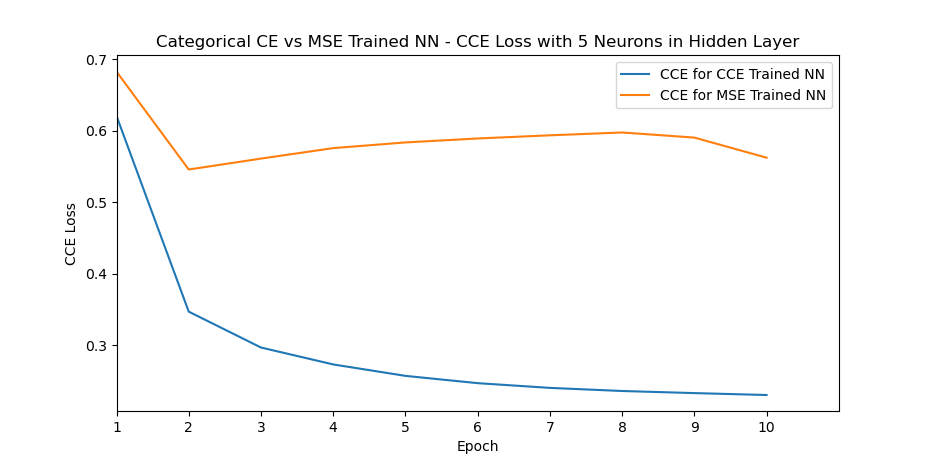
\includegraphics[width=\textwidth]{1. CCE vs MSE - CCE Loss - 5 Neurons.png}
	\caption{Γραφική Παράσταση σύγκλισης με χρήση Categorical CE vs MSE συνάρτηση σφάλματος και 5 νευρώνες στο κρυφό επίπεδο}
\end{figure}

\begin{figure}[H]
	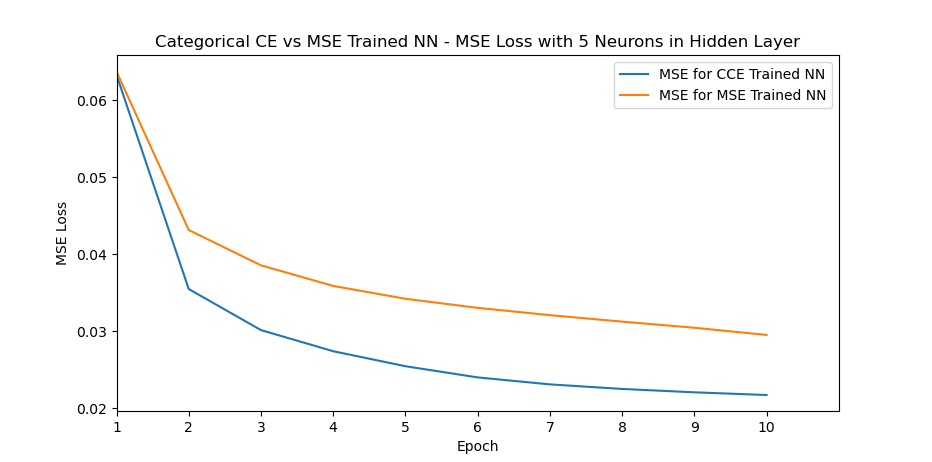
\includegraphics[width=\textwidth]{2. CCE vs MSE - MSE Loss - 5 Neurons.png}
	\caption{Γραφική Παράσταση σύγκλισης με χρήση Categorical CE vs MSE συνάρτηση σφάλματος και 5 νευρώνες στο κρυφό επίπεδο}
\end{figure}

\begin{figure}[H]
	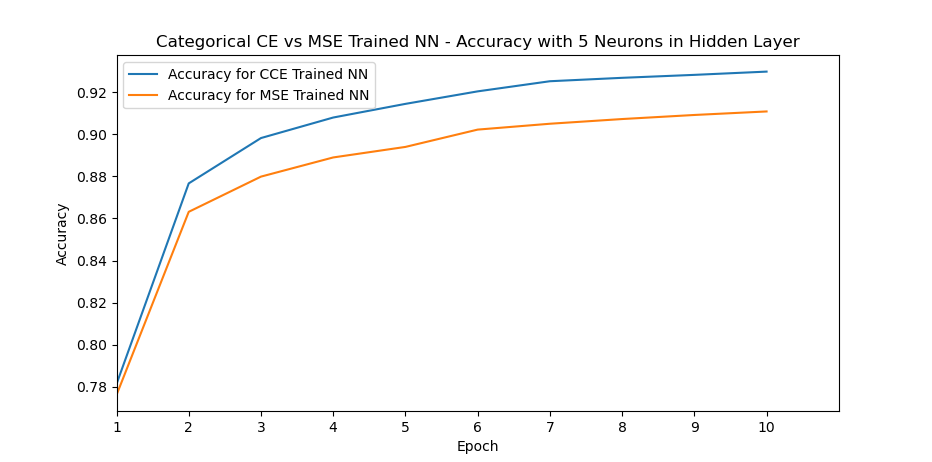
\includegraphics[width=\textwidth]{3. CCE vs MSE - Accuracy - 5 Neurons.png}
	\caption{Γραφική Παράσταση σύγκλισης με χρήση Categorical CE vs MSE συνάρτηση σφάλματος και 5 νευρώνες στο κρυφό επίπεδο}
\end{figure}

\textbf{Με 12 νευρώνες στο κρυφό επίπεδο:}

\begin{figure}[H]
	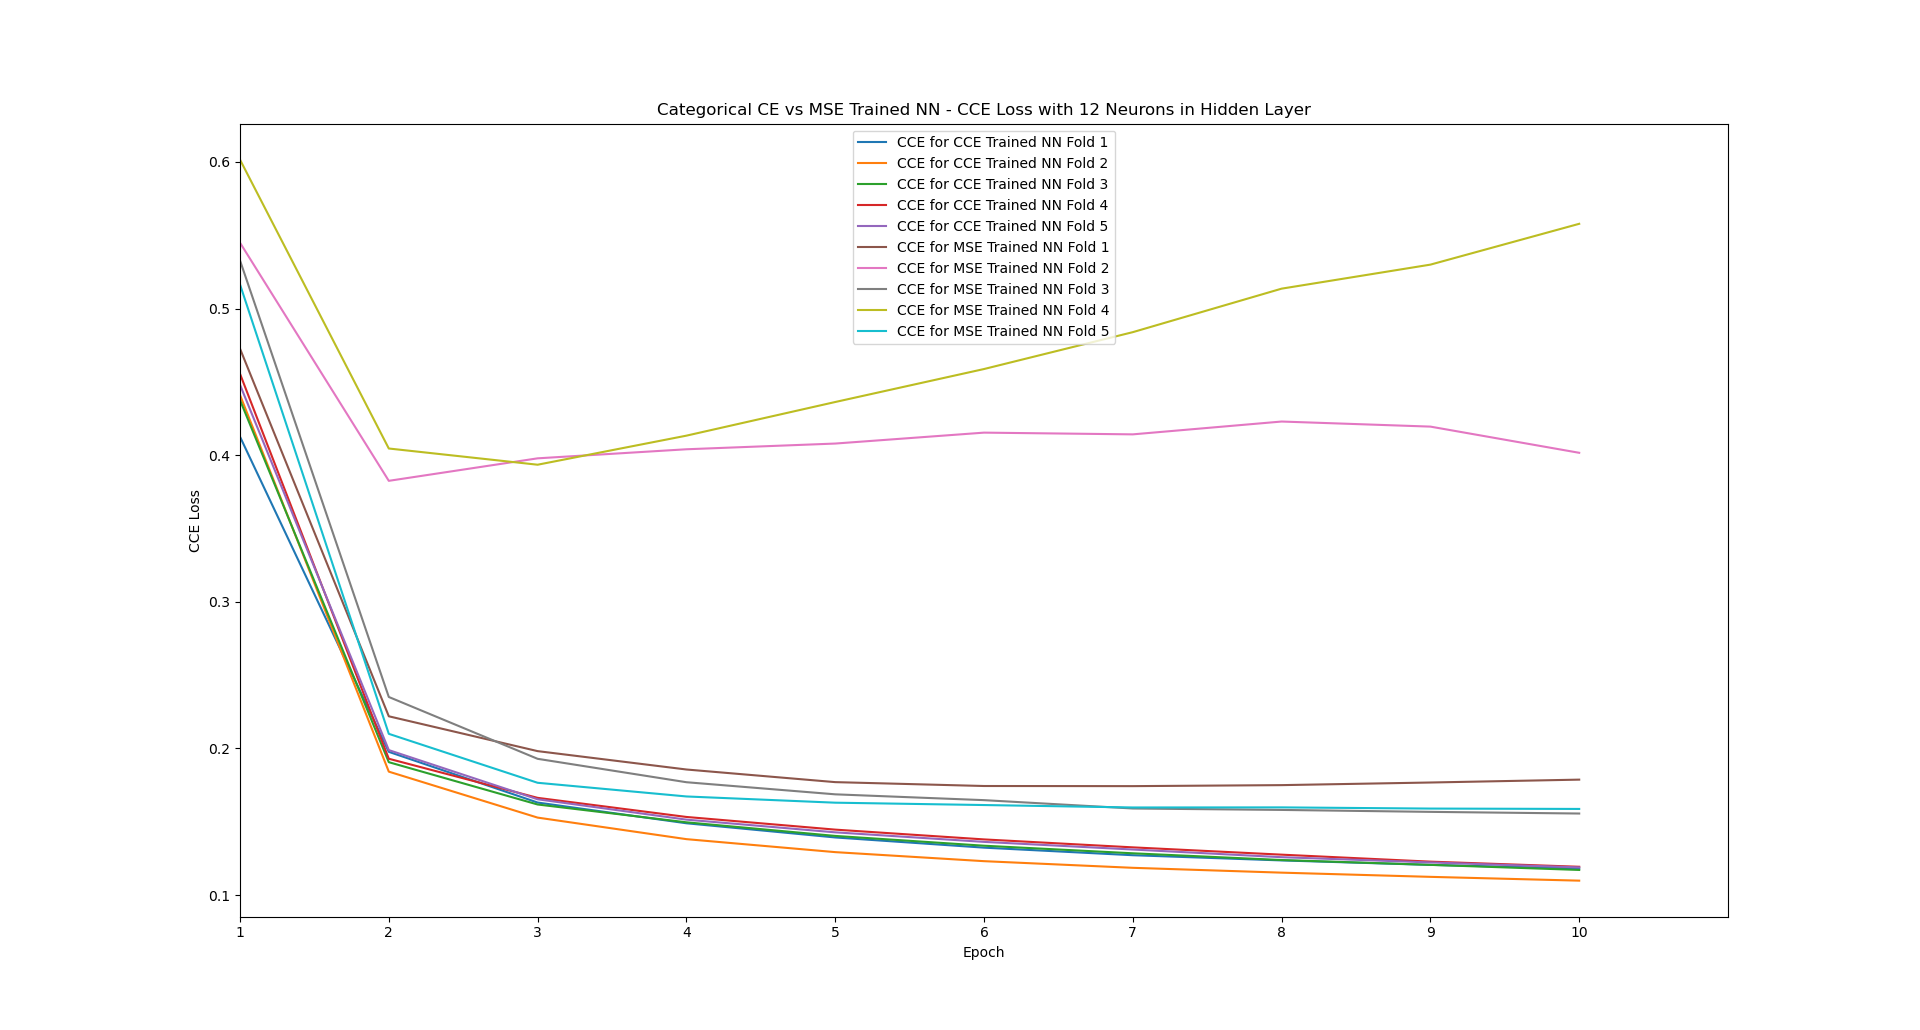
\includegraphics[width=\textwidth]{4. CCE vs MSE - CCE Loss - 12 Neurons.png}
	\caption{Γραφική Παράσταση σύγκλισης με χρήση Categorical CE vs MSE συνάρτηση σφάλματος και 12 νευρώνες στο κρυφό επίπεδο}
\end{figure}

\begin{figure}[H]
	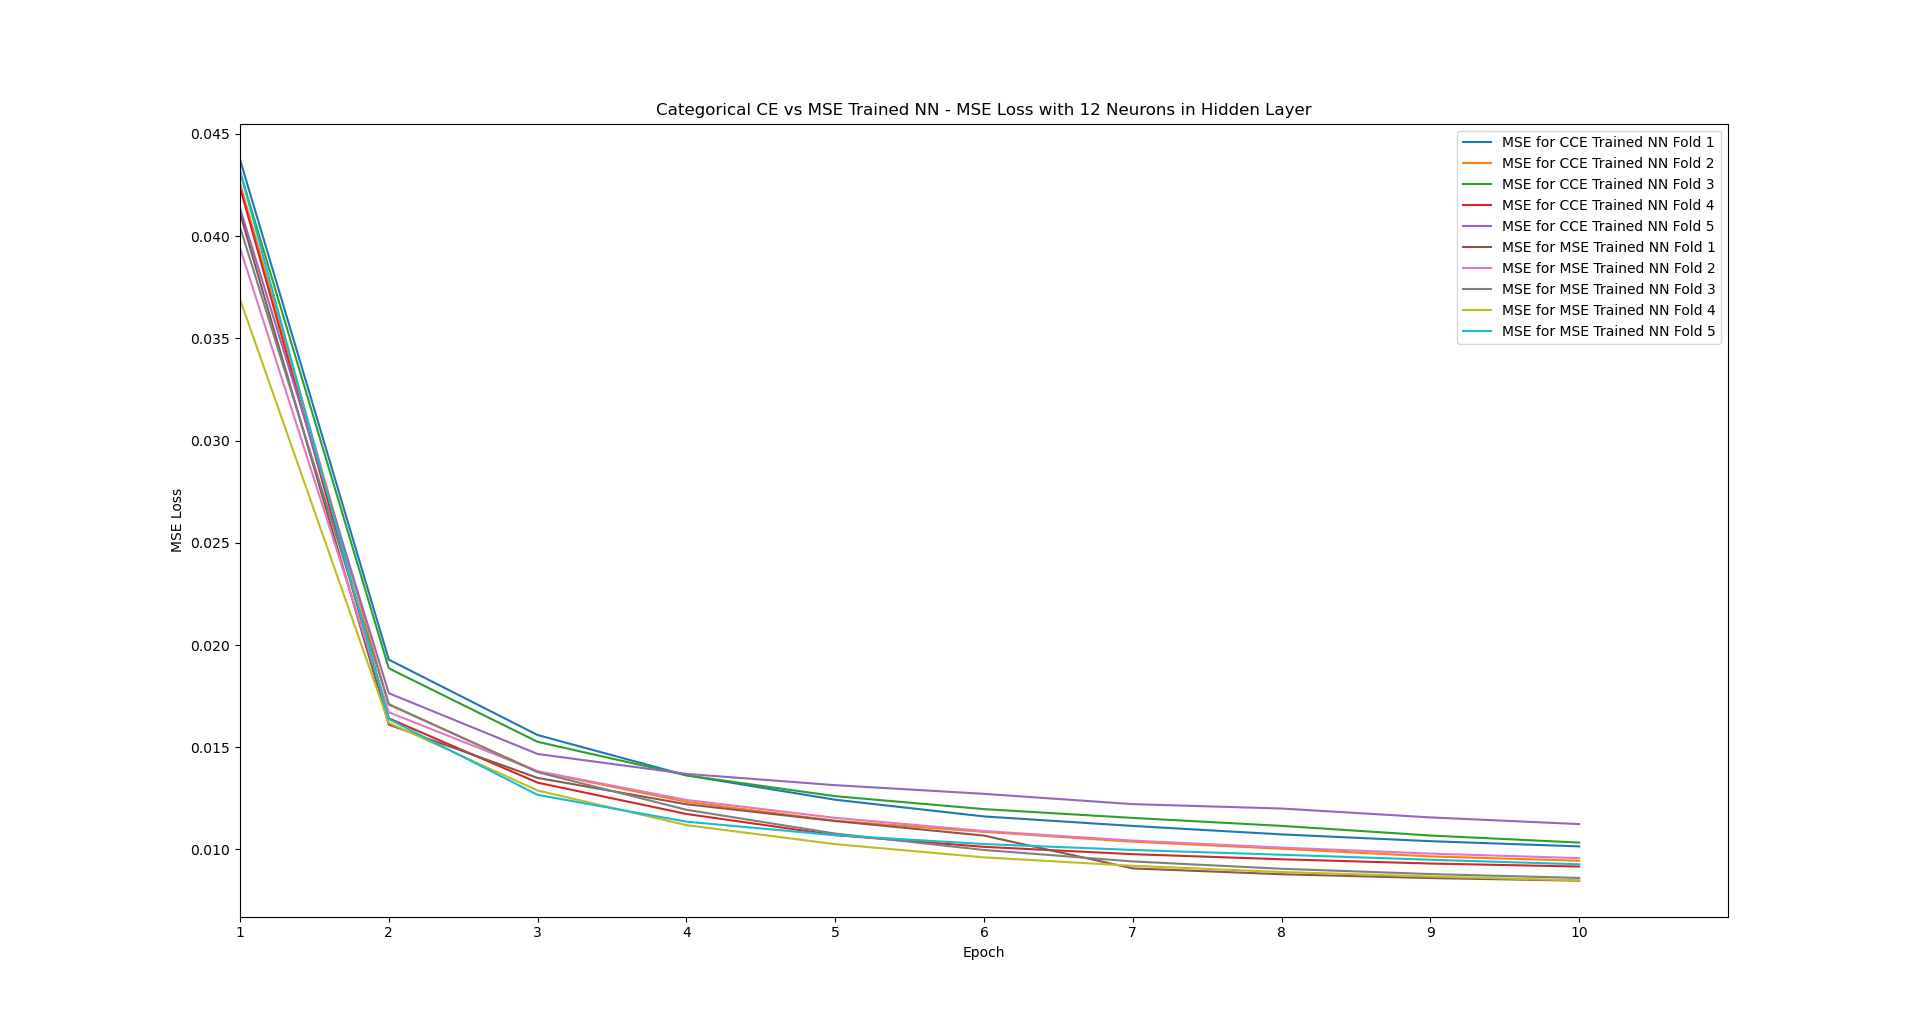
\includegraphics[width=\textwidth]{5. CCE vs MSE - MSE Loss - 12 Neurons.png}
	\caption{Γραφική Παράσταση σύγκλισης με χρήση Categorical CE vs MSE συνάρτηση σφάλματος και 12 νευρώνες στο κρυφό επίπεδο}
\end{figure}

\begin{figure}[H]
	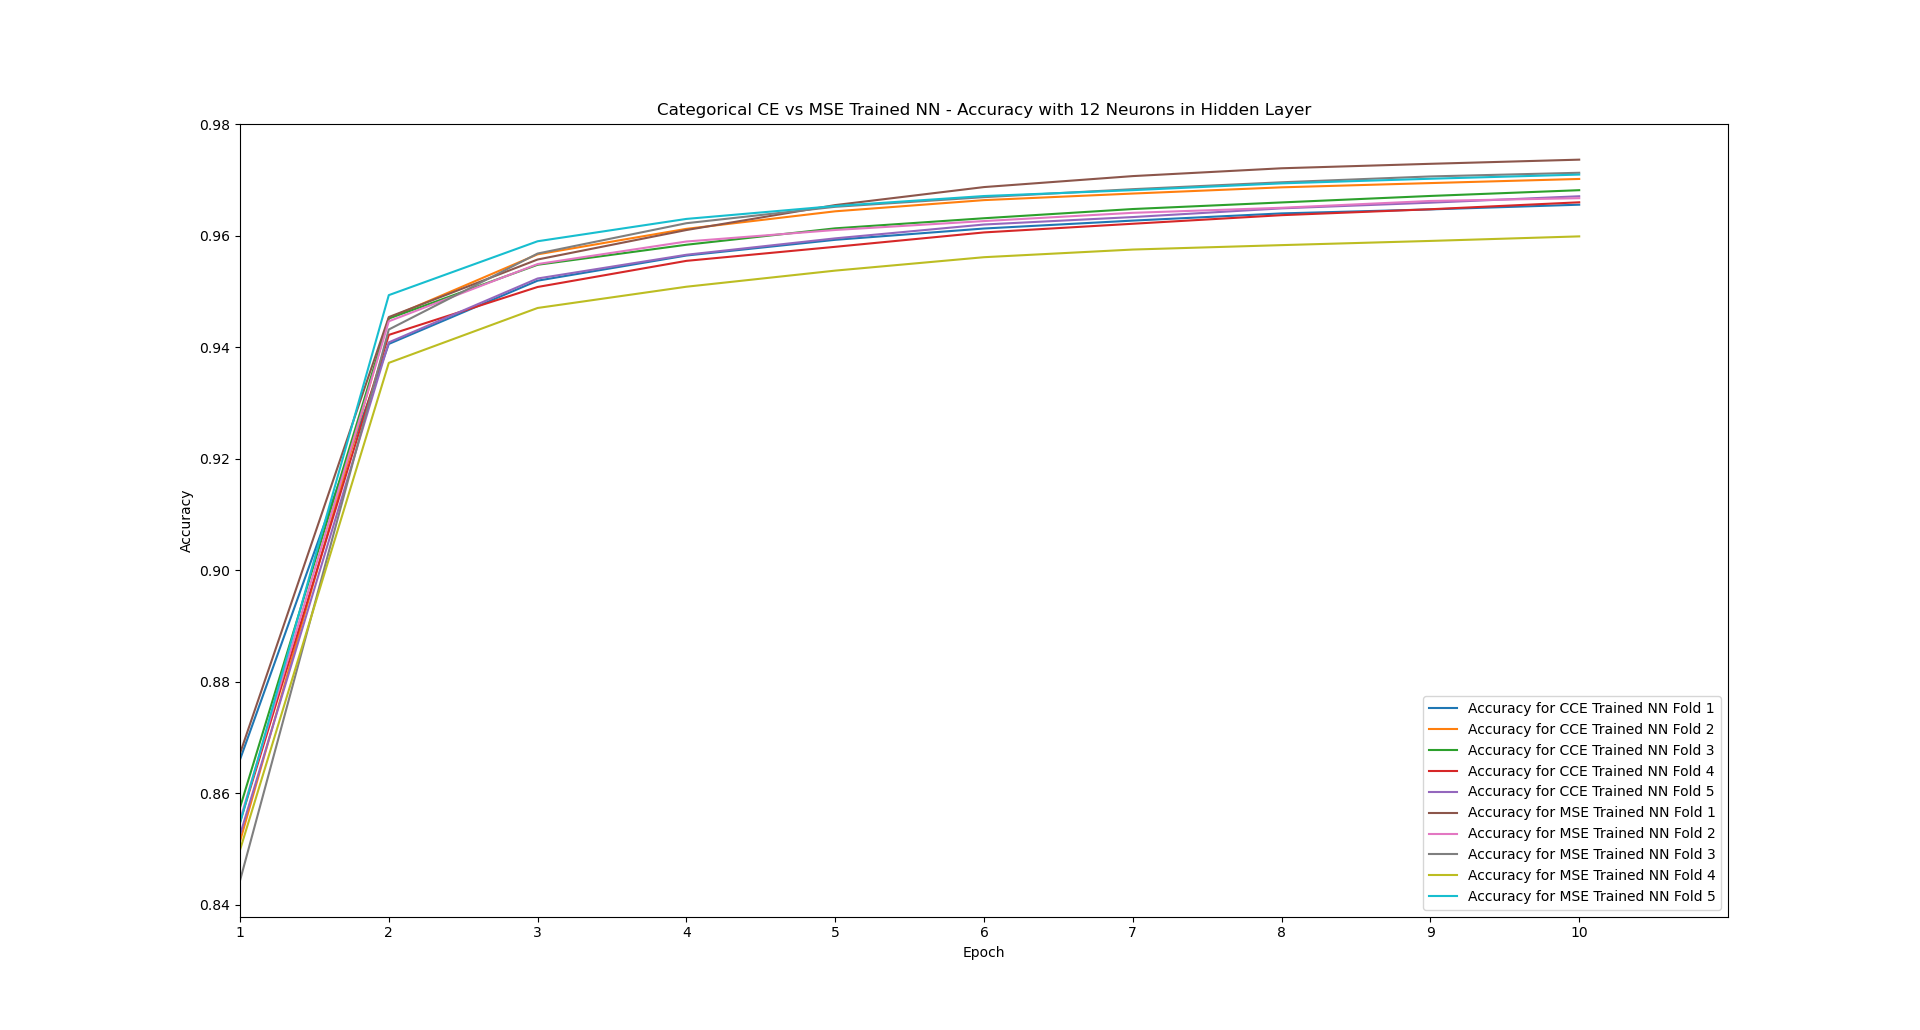
\includegraphics[width=\textwidth]{6. CCE vs MSE - Accuracy - 12 Neurons.png}
	\caption{Γραφική Παράσταση σύγκλισης με χρήση Categorical CE vs MSE συνάρτηση σφάλματος και 12 νευρώνες στο κρυφό επίπεδο}
\end{figure}

\textbf{Με 23 νευρώνες στο κρυφό επίπεδο:}

\begin{figure}[H]
	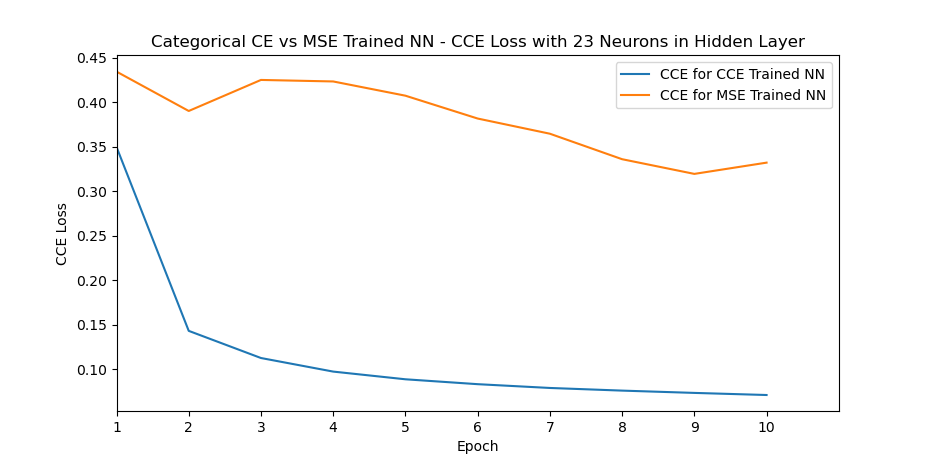
\includegraphics[width=\textwidth]{7. CCE vs MSE - CCE Loss - 23 Neurons.png}
	\caption{Γραφική Παράσταση σύγκλισης με χρήση Categorical CE vs MSE συνάρτηση σφάλματος και 23 νευρώνες στο κρυφό επίπεδο}
\end{figure}

\begin{figure}[H]
	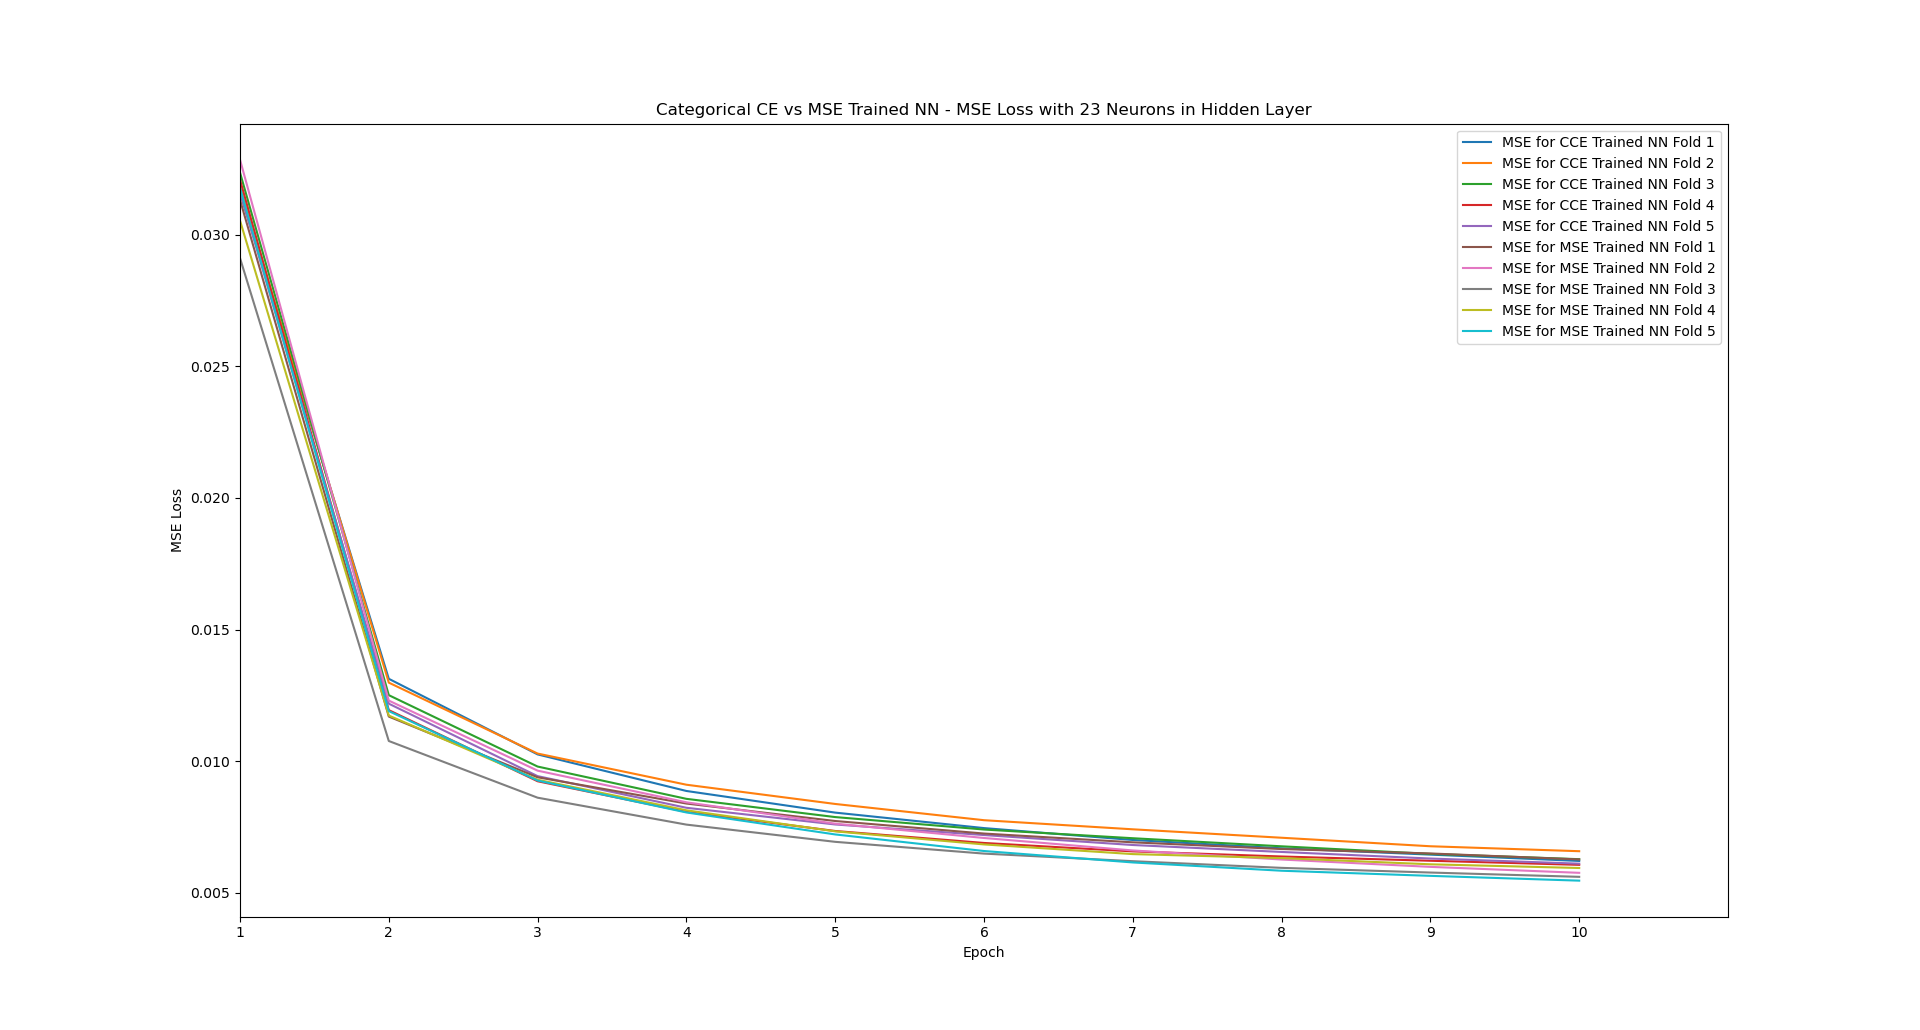
\includegraphics[width=\textwidth]{8. CCE vs MSE - MSE Loss - 23 Neurons.png}
	\caption{Γραφική Παράσταση σύγκλισης με χρήση Categorical CE vs MSE συνάρτηση σφάλματος και 23 νευρώνες στο κρυφό επίπεδο}
\end{figure}

\begin{figure}[H]
	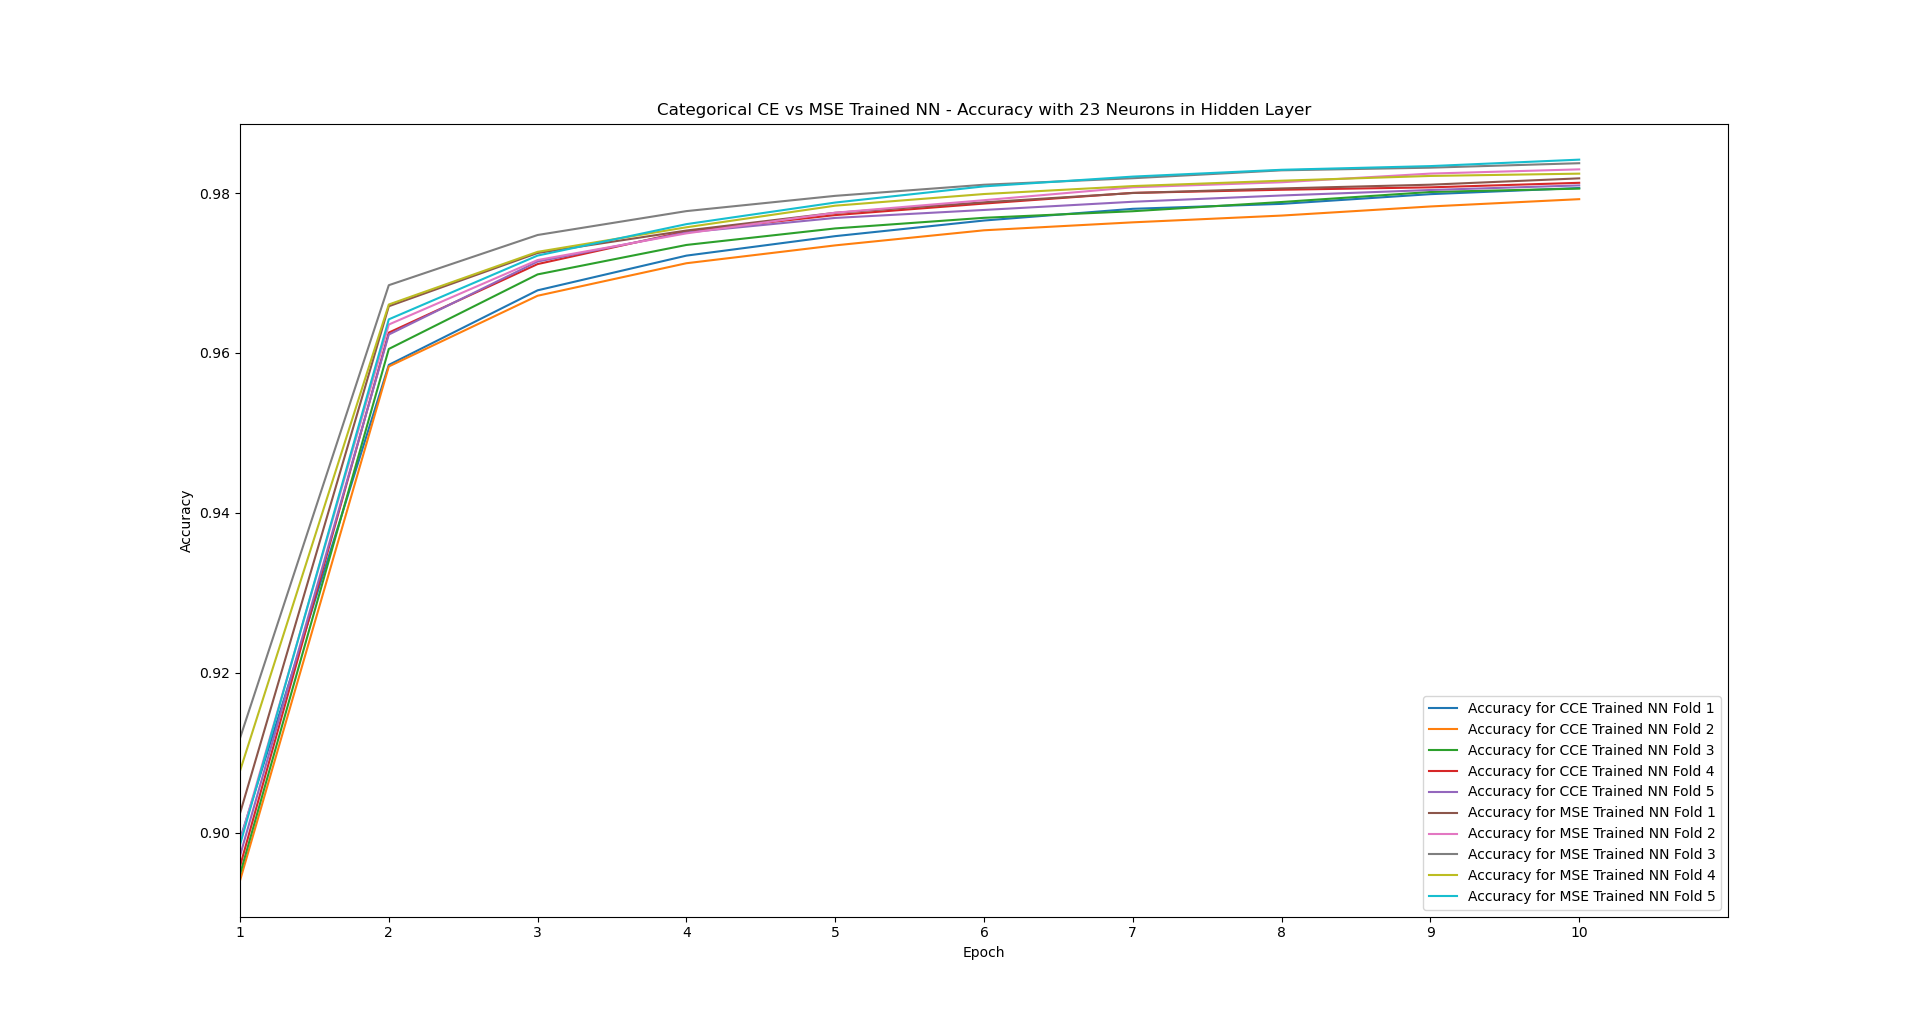
\includegraphics[width=\textwidth]{9. CCE vs MSE - Accuracy - 23 Neurons.png}
	\caption{Γραφική Παράσταση σύγκλισης με χρήση Categorical CE vs MSE συνάρτηση σφάλματος και 23 νευρώνες στο κρυφό επίπεδο}
\end{figure}

\subsubsection{Συμπεράσματα}

\begin{enumerate}
    \item Σχετικά με τον αριθμό των κρυφών κόμβων παρατηρώ πως ανεξάρτητα από τη συνάρτηση κόστους που χρησιμοποιείται στην εκπαίδευση, ο μεγαλύτερος αριθμός κόμβων οδηγεί σε μικρότερες τιμές των μετρικών σφαλμάτων και μεγαλύτερη τιμή της μετρικής Accuracy. Άρα με περισσότερους κρυφούς κόμβους η απόδοση του ΤΝΔ είναι καλύτερη.
    \item Σχετικά με τη συνάρτηση κόστους παρατηρώ ότι η εκπαίδευση μέσω Categorical CE φέρει καλύτερα αποτελέσματα, όπως ήταν αναμενόμενο για τους λόγους που αναφέρθηκαν στο κεφάλαιο \ref{Ανάλυση Μετρικών}.
    \item Παρατηρώ πως όταν χρησιμοποιώ την αποδοτικότερη συνάρτηση κόστους, δηλαδή την Categorical CE, όσο μεγαλώνει ο αριθμός των εποχών τόσο μικρότερη γίνεται η κλήση μείωσης του σφάλματος και αύξησης του Accuracy. Αυτή η συμπεριφορά προκύπτει από τον αλγόριθμο gradient descent που χρησιμοποιούμε για την εύρεση των βέλτιστων βαρών δηλαδή αυτά που επιτελούν το ελάχιστο κόστος (και με έμμεσο τρόπο τη μέγιστη ακρίβεια).
\end{enumerate}

\end{document}
